\chapter{نظریه اعداد}

\index{نظریه اعداد}

\key{نظریه اعداد} شاخه‌ای از ریاضیات است
که به مطالعه اعداد صحیح می‌پردازد.
نظریه اعداد حوزه‌ای شگفت‌انگیز است،
چرا که بسیاری از پرسش‌های مربوط به اعداد صحیح،
حتی اگر در نگاه اول ساده به نظر برسند،
حل بسیار دشواری دارند.

به عنوان مثال، معادله زیر را در نظر بگیرید:
\[x^3 + y^3 + z^3 = 33\]
یافتن سه عدد حقیقی $x$، $y$ و $z$
که در این معادله صدق کنند آسان است.
برای نمونه می‌توان انتخاب کرد:
\[
\begin{array}{lcl}
x = 3, \\
y = \sqrt[3]{3}, \\
z = \sqrt[3]{3}.\\
\end{array}
\]
با این حال، در نظریه اعداد این مسئله‌ای باز است
که آیا سه \emph{عدد صحیح} $x$، $y$ و $z$ وجود دارند
که در این معادله صدق کنند یا خیر \cite{bec07}.

در این فصل، روی مفاهیم پایه
و الگوریتم‌های نظریه اعداد تمرکز خواهیم کرد.
در سرتاسر این فصل، فرض بر این است که همه اعداد
صحیح هستند، مگر خلاف آن بیان شود.

\section{اعداد اول و مقسوم‌علیه‌ها}

\index{بخش‌پذیری}
\index{عامل}
\index{مقسوم‌علیه}

عدد $a$ را یک \key{عامل} یا \key{مقسوم‌علیه} عدد $b$ می‌نامند
هرگاه $a$ عدد $b$ را عاد کند (تقسیم کند).
اگر $a$ مقسوم‌علیه $b$ باشد،
می‌نویسیم $a \mid b$، و در غیر این صورت می‌نویسیم $a \nmid b$.
برای مثال، مقسوم‌علیه‌های 24 عبارتند از:
1، 2، 3، 4، 6، 8، 12 و 24.

\index{عدد اول}
\index{تجزیه به عوامل اول}

عدد $n>1$ یک \key{عدد اول} است
اگر تنها مقسوم‌علیه‌های مثبت آن 1 و $n$ باشند.
برای نمونه، 7، 19 و 41 اول هستند،
اما 35 اول نیست، زیرا $5 \cdot 7 = 35$.
به ازای هر عدد $n>1$، یک \key{تجزیه به عوامل اول} یکتا وجود دارد:
\[ n = p_1^{\alpha_1} p_2^{\alpha_2} \cdots p_k^{\alpha_k},\]
که در آن $p_1,p_2,\ldots,p_k$ اعداد اول متمایز و
$\alpha_1,\alpha_2,\ldots,\alpha_k$ اعداد مثبت هستند.
برای مثال، تجزیه به عوامل اول برای 84 به صورت زیر است:
\[84 = 2^2 \cdot 3^1 \cdot 7^1.\]

\key{تعداد مقسوم‌علیه‌ها}ی عدد $n$ برابر است با:
\[\tau(n)=\prod_{i=1}^k (\alpha_i+1),\]
زیرا برای هر عامل اول $p_i$، به تعداد $\alpha_i+1$
روش برای انتخاب تعداد دفعات حضور آن
در مقسوم‌علیه وجود دارد.
برای مثال، تعداد مقسوم‌علیه‌های 84 برابر است با:
$\tau(84)=3 \cdot 2 \cdot 2 = 12$.
این مقسوم‌علیه‌ها عبارتند از:
1، 2، 3، 4، 6، 7، 12، 14، 21، 28، 42 و 84.

\key{مجموع مقسوم‌علیه‌ها}ی $n$ برابر است با:
\[\sigma(n)=\prod_{i=1}^k (1+p_i+\ldots+p_i^{\alpha_i}) = \prod_{i=1}^k \frac{p_i^{a_i+1}-1}{p_i-1},\]
که در آن، فرمول دوم بر اساس فرمول تصاعد هندسی به دست آمده است.
برای مثال، مجموع مقسوم‌علیه‌های 84 برابر است با:
\[\sigma(84)=\frac{2^3-1}{2-1} \cdot \frac{3^2-1}{3-1} \cdot \frac{7^2-1}{7-1} = 7 \cdot 4 \cdot 8 = 224.\]

\key{حاصل‌ضرب مقسوم‌علیه‌ها}ی $n$ برابر است با:
\[\mu(n)=n^{\tau(n)/2},\]
زیرا می‌توان از میان مقسوم‌علیه‌ها $\tau(n)/2$ جفت تشکیل داد
که حاصل‌ضرب هر جفت برابر با $n$ است.
برای نمونه، مقسوم‌علیه‌های 84 این جفت‌ها را می‌سازند:
$1 \cdot 84$، $2 \cdot 42$، $3 \cdot 28$ و غیره،
و حاصل‌ضرب مقسوم‌علیه‌ها برابر است با: $\mu(84)=84^6=351298031616$.

\index{عدد کامل}

عدد $n$ یک \key{عدد کامل} نامیده می‌شود اگر $n=\sigma(n)-n$ باشد؛
یعنی $n$ برابر با مجموع مقسوم‌علیه‌های خود
بین $1$ و $n-1$ باشد.
برای مثال، 28 یک عدد کامل است،
زیرا $28=1+2+4+7+14$.

\subsubsection{تعداد اعداد اول}

نشان دادن نامتناهی بودن اعداد اول ساده است.
اگر تعداد اعداد اول متناهی بود،
مجموعه $P=\{p_1,p_2,\ldots,p_n\}$
شامل همه اعداد اول تشکیل می‌شد.
مثال: $p_1=2$، $p_2=3$، $p_3=5$ و الی آخر.
ولی با اعضای $P$، عدد اول جدید
\[p_1 p_2 \cdots p_n+1\]
ساخته می‌شود
که از تمام اعضای $P$ بزرگ‌تر است.
این تناقض است. تعداد اعداد اول باید نامتناهی باشد.

\subsubsection{تراکم اعداد اول}

تراکم اعداد اول یعنی بسامد رخداد اعداد اول میان اعداد.
فرض کنید $\pi(n)$ نماد تعداد اعداد اول بین
$1$ و $n$ باشد. مثال: $\pi(10)=4$، چون
۴ عدد اول بین $1$ و $10$ هست: 2، 3، 5 و 7.

می‌توان نشان داد
\[\pi(n) \approx \frac{n}{\ln n},\]
یعنی اعداد اول متداول هستند.
مثال: تعداد اعداد اول بین
$1$ و $10^6$ برابر $\pi(10^6)=78498$ است،
و $10^6 / \ln 10^6 \approx 72382$.

\subsubsection{حدس‌ها}

\emph{حدس‌های} زیادی درباره اعداد اول وجود دارد.
اکثر افراد حدس‌ها را درست می‌دانند،
اما اثباتی برای آن‌ها نیست.
حدس‌های مشهور:

\begin{itemize}
\index{حدس گلدباخ}
\item \key{حدس گلدباخ}:
هر عدد صحیح زوج $n>2$ به شکل
مجموع $n=a+b$ نوشته می‌شود که هر دو عدد $a$ و $b$ اول هستند.
\index{اعداد اول دوقلو}
\item \key{حدس اعداد اول دوقلو}:
تعداد نامتناهی جفت
به فرم $\{p,p+2\}$ وجود دارد
که در آن هم $p$ و هم $p+2$ اول هستند.
\index{حدس لژاندر}
\item \key{حدس لژاندر}:
همیشه یک عدد اول بین
$n^2$ و $(n+1)^2$ هست، که $n$ هر عدد صحیح مثبت است.
\end{itemize}

\subsubsection{الگوریتم‌های پایه}

اگر عدد $n$ اول نباشد،
به صورت حاصل‌ضرب $a \cdot b$ نوشته می‌شود،
که $a \le \sqrt n$ یا $b \le \sqrt n$ است،
پس قطعا عاملی بین $2$ و $\lfloor \sqrt n \rfloor$ دارد.
با این نکته، تست اول بودن عدد
و تجزیه به عوامل اول در زمان $O(\sqrt n)$ انجام می‌شود.

تابع \texttt{prime} بررسی می‌کند
آیا عدد ورودی $n$ اول است یا خیر.
تابع تقسیم $n$ بر
تمام اعداد بین $2$ و $\lfloor \sqrt n \rfloor$ را امتحان می‌کند،
و اگر هیچ‌کدام $n$ را عاد نکند، $n$ اول است.

\begin{lstlisting}
bool prime(int n) {
    if (n < 2) return false;
    for (int x = 2; x*x <= n; x++) {
        if (n%x == 0) return false;
    }
    return true;
}
\end{lstlisting}

\noindent
تابع \texttt{factors}
یک بردار شامل عوامل اول $n$
می‌سازد.
تابع $n$ را بر عوامل اولش تقسیم می‌کند،
و آن‌ها را به بردار می‌افزاید.
فرایند زمانی پایان می‌یابد که عدد باقی‌مانده $n$
عاملی بین $2$ و $\lfloor \sqrt n \rfloor$ نداشته باشد.
اگر $n>1$، اول است و آخرین عامل خواهد بود.

\begin{lstlisting}
vector<int> factors(int n) {
    vector<int> f;
    for (int x = 2; x*x <= n; x++) {
        while (n%x == 0) {
            f.push_back(x);
            n /= x;
        }
    }
    if (n > 1) f.push_back(n);
    return f;
}
\end{lstlisting}

توجه کنید هر عامل اول به تعداد دفعاتی که عدد را عاد می‌کند در بردار ظاهر می‌شود.
برای مثال، $24=2^3 \cdot 3$،
بنابراین خروجی تابع $[2,2,2,3]$ است.

\subsubsection{غربال اراتستن}

\index{غربال اراتستن}

\key{غربال اراتستن}
%\footnote{Eratosthenes (c. 276 BC -- c. 194 BC) was a Greek mathematician.}
الگوریتم پیش‌پردازشی است که آرایه‌ای می‌سازد. با این آرایه می‌توان اول بودن هر عدد دلخواه بین $2 \ldots n$ را به‌طور کارآمد بررسی کرد و در صورت اول نبودن، یکی از عامل‌های اول آن را یافت.

این الگوریتم آرایه‌ای به نام $\texttt{sieve}$ می‌سازد که خانه‌های $2,3,\ldots,n$ آن استفاده می‌شوند.
مقدار $\texttt{sieve}[k]=0$ یعنی $k$ اول است،
و مقدار $\texttt{sieve}[k] \neq 0$ یعنی $k$ مرکب است و یکی از عامل‌های اول آن $\texttt{sieve}[k]$ است.

الگوریتم اعداد $2 \ldots n$ را تک‌به‌تک پیمایش می‌کند.
هر بار با یافتن عدد اول جدید $x$، مضرب‌های آن ($2x,3x,4x,\ldots$) را به عنوان عدد غیر اول علامت‌گذاری می‌کند، چون عدد $x$ آنها را عاد می‌کند.

برای مثال، اگر $n=20$ باشد، آرایه به این صورت است:

\begin{center}
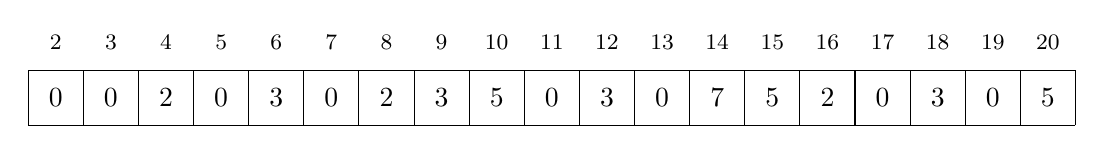
\begin{tikzpicture}[scale=0.7]
\draw (0,0) grid (19,1);

\node at (0.5,0.5) {$0$};
\node at (1.5,0.5) {$0$};
\node at (2.5,0.5) {$2$};
\node at (3.5,0.5) {$0$};
\node at (4.5,0.5) {$3$};
\node at (5.5,0.5) {$0$};
\node at (6.5,0.5) {$2$};
\node at (7.5,0.5) {$3$};
\node at (8.5,0.5) {$5$};
\node at (9.5,0.5) {$0$};
\node at (10.5,0.5) {$3$};
\node at (11.5,0.5) {$0$};
\node at (12.5,0.5) {$7$};
\node at (13.5,0.5) {$5$};
\node at (14.5,0.5) {$2$};
\node at (15.5,0.5) {$0$};
\node at (16.5,0.5) {$3$};
\node at (17.5,0.5) {$0$};
\node at (18.5,0.5) {$5$};

\footnotesize

\node at (0.5,1.5) {$2$};
\node at (1.5,1.5) {$3$};
\node at (2.5,1.5) {$4$};
\node at (3.5,1.5) {$5$};
\node at (4.5,1.5) {$6$};
\node at (5.5,1.5) {$7$};
\node at (6.5,1.5) {$8$};
\node at (7.5,1.5) {$9$};
\node at (8.5,1.5) {$10$};
\node at (9.5,1.5) {$11$};
\node at (10.5,1.5) {$12$};
\node at (11.5,1.5) {$13$};
\node at (12.5,1.5) {$14$};
\node at (13.5,1.5) {$15$};
\node at (14.5,1.5) {$16$};
\node at (15.5,1.5) {$17$};
\node at (16.5,1.5) {$18$};
\node at (17.5,1.5) {$19$};
\node at (18.5,1.5) {$20$};

\end{tikzpicture}
\end{center}

کد زیر غربال اراتستن را پیاده‌سازی می‌کند.
کد فرض می‌کند تمام عناصر $\texttt{sieve}$ در ابتدا صفر هستند.

\begin{lstlisting}
for (int x = 2; x <= n; x++) {
    if (sieve[x]) continue;
    for (int u = 2*x; u <= n; u += x) {
        sieve[u] = x;
    }
}
\end{lstlisting}

حلقه داخلی الگوریتم به ازای هر مقدار $x$،
به تعداد $n/x$ بار اجرا می‌شود.
بنابراین، یک کران بالا برای زمان اجرای
الگوریتم، مجموع هارمونیک زیر است:
\[\sum_{x=2}^n n/x = n/2 + n/3 + n/4 + \cdots + n/n = O(n \log n).\]

\index{harmonic sum@مجموع هارمونیک}

در واقع، الگوریتم کارآمدتر است،
زیرا حلقه داخلی تنها زمانی اجرا می‌شود که
عدد $x$ اول باشد.
می‌توان نشان داد که زمان اجرای
الگوریتم تنها $O(n \log \log n)$ است؛
پیچیدگی زمانی بسیار نزدیکی به $O(n)$.

\subsubsection{الگوریتم اقلیدس}

\index{greatest common divisor@بزرگ‌ترین مقسوم‌علیه مشترک}
\index{least common multiple@کوچک‌ترین مضرب مشترک}
\index{Euclid's algorithm@الگوریتم اقلیدس}

\key{بزرگ‌ترین مقسوم‌علیه مشترک}
دو عدد $a$ و $b$، یعنی $\gcd(a,b)$،
بزرگ‌ترین عددی است که هر دو عدد $a$ و $b$ را عاد می‌کند،
و \key{کوچک‌ترین مضرب مشترک}
$a$ و $b$، یعنی $\textrm{lcm}(a,b)$،
کوچک‌ترین عددی است که بر
هر دوی $a$ و $b$ بخش‌پذیر است.
به عنوان مثال،
$\gcd(24,36)=12$ و
$\textrm{lcm}(24,36)=72$.

بزرگ‌ترین مقسوم‌علیه مشترک و کوچک‌ترین مضرب مشترک
به شکل زیر به هم مرتبط هستند:
\[\textrm{lcm}(a,b)=\frac{ab}{\textrm{gcd}(a,b)}\]

\key{الگوریتم اقلیدس}\footnote{اقلیدس ریاضی‌دانی یونانی بود که
حدود ۳۰۰ سال پیش از میلاد می‌زیست. این احتمالاً نخستین الگوریتم شناخته‌شده در تاریخ است.} روشی کارآمد برای
یافتن بزرگ‌ترین مقسوم‌علیه مشترک دو عدد فراهم می‌کند.
این الگوریتم مبتنی بر فرمول زیر است:
\begin{equation*}
    \textrm{gcd}(a,b) = \begin{cases}
               a        & b = 0\\
               \textrm{gcd}(b,a \bmod b) & b \neq 0\\
           \end{cases}
\end{equation*}

برای نمونه،
\[\textrm{gcd}(24,36) = \textrm{gcd}(36,24)
= \textrm{gcd}(24,12) = \textrm{gcd}(12,0)=12.\]

الگوریتم را می‌توان به صورت زیر پیاده‌سازی کرد:
\begin{lstlisting}
int gcd(int a, int b) {
    if (b == 0) return a;
    return gcd(b, a%b);
}
\end{lstlisting}

می‌توان نشان داد که الگوریتم اقلیدس در زمان
$O(\log n)$ اجرا می‌شود که در آن $n=\min(a,b)$ است.
بدترین حالت برای این الگوریتم،
زمانی رخ می‌دهد که $a$ و $b$ دو عدد متوالی فیبوناچی باشند.
برای نمونه،
\[\textrm{gcd}(13,8)=\textrm{gcd}(8,5)
=\textrm{gcd}(5,3)=\textrm{gcd}(3,2)=\textrm{gcd}(2,1)=\textrm{gcd}(1,0)=1.\]

\subsubsection{تابع فی اویلر}

\index{coprime@نسبت به هم اول}
\index{Euler's totient function@تابع فی اویلر}

دو عدد $a$ و $b$ را \key{متباین} (نسبت به هم اول) می‌نامند
اگر $\textrm{gcd}(a,b)=1$ باشد.
\key{تابع فی اویلر} $\varphi(n)$
%\footnote{اویلر این تابع را در سال ۱۷۶۳ معرفی کرد.}
تعداد اعداد متباین با $n$
را در بازهٔ $1$ تا $n$ به دست می‌دهد.
برای نمونه، $\varphi(12)=4$،
زیرا اعداد ۱، ۵، ۷ و ۱۱
نسبت به ۱۲ اول هستند.

مقدار $\varphi(n)$ را می‌توان از روی
تجزیه $n$ به عوامل اول
با استفاده از فرمول زیر محاسبه کرد:
\[ \varphi(n) = \prod_{i=1}^k p_i^{\alpha_i-1}(p_i-1). \]
برای نمونه، $\varphi(12)=2^1 \cdot (2-1) \cdot 3^0 \cdot (3-1)=4$.
دقت کنید که اگر $n$ اول باشد، $\varphi(n)=n-1$ خواهد بود.

\section{حساب پیمانه‌ای}

\index{modular arithmetic@حساب پیمانه‌ای}

در \key{حساب پیمانه‌ای}،
مجموعه اعداد به گونه‌ای محدود می‌شود که
تنها اعداد $0,1,2,\ldots,m-1$ به کار می‌روند؛
جایی که $m$ یک عدد ثابت است.
هر عدد $x$ با
عدد $x \bmod m$ نشان داده می‌شود:
باقی‌مانده تقسیم $x$ بر $m$.
برای نمونه، اگر $m=17$ باشد، عدد $75$
به صورت $75 \bmod 17 = 7$ نشان داده می‌شود.

اغلب می‌توان پیش از انجام محاسبات،
باقی‌مانده را محاسبه کرد.
به ویژه، روابط زیر برقرار هستند:
\[
\begin{array}{rcl}
(x+y) \bmod m & = & (x \bmod m + y \bmod m) \bmod m \\
(x-y) \bmod m & = & (x \bmod m - y \bmod m) \bmod m \\
(x \cdot y) \bmod m & = & (x \bmod m \cdot y \bmod m) \bmod m \\
x^n \bmod m & = & (x \bmod m)^n \bmod m \\
\end{array}
\]

\subsubsection{توان‌رسانی پیمانه‌ای}

اغلب نیاز است مقدار $x^n \bmod m$
به شکل کارآمد محاسبه شود.
این کار را می‌توان در زمان $O(\log n)$
و با استفاده از رابطه بازگشتی زیر انجام داد:
\begin{equation*}
    x^n = \begin{cases}
               1        & n = 0\\
               x^{n/2} \cdot x^{n/2} & \text{$n$ زوج است}\\
               x^{n-1} \cdot x & \text{$n$ فرد است}
           \end{cases}
\end{equation*}

مهم است که در حالت $n$ زوج،
مقدار $x^{n/2}$ تنها یک بار محاسبه شود.
این امر تضمین می‌کند که پیچیدگی زمانی الگوریتم
برابر $O(\log n)$ باشد، چرا که $n$ در صورت زوج بودن همواره نصف می‌شود.

تابع زیر مقدار $x^n \bmod m$ را محاسبه می‌کند:

\begin{lstlisting}
int modpow(int x, int n, int m) {
    if (n == 0) return 1%m;
    long long u = modpow(x,n/2,m);
    u = (u*u)%m;
    if (n%2 == 1) u = (u*x)%m;
    return u;
}
\end{lstlisting}

\subsubsection{قضیه فرما و قضیه اویلر}

\index{قضیه فرما}
\index{قضیه اویلر}

\key{قضیه فرما}
%\footnote{فرما این قضیه را در سال ۱۶۴۰ کشف کرد.}
بیان می‌کند که
\[x^{m-1} \bmod m = 1\]
وقتی که $m$ اول باشد و $x$ و $m$ نسبت به هم اول باشند.
همچنین نتیجه می‌دهد:
\[x^k \bmod m = x^{k \bmod (m-1)} \bmod m.\]
در حالتی کلی‌تر، \key{قضیه اویلر}
%\footnote{اویلر این قضیه را در سال ۱۷۶۳ منتشر کرد.}
بیان می‌کند که
\[x^{\varphi(m)} \bmod m = 1\]
وقتی که $x$ و $m$ نسبت به هم اول باشند.
قضیه فرما از قضیه اویلر به دست می‌آید،
زیرا اگر $m$ عددی اول باشد، $\varphi(m)=m-1$ خواهد بود.

\subsubsection{معکوس پیمانه‌ای}

\index{معکوس پیمانه‌ای}

معکوس $x$ به پیمانه $m$
عددی مانند $x^{-1}$ است به طوری که:
\[ x x^{-1} \bmod m = 1. \]
برای نمونه، اگر $x=6$ و $m=17$ باشد،
آن‌گاه $x^{-1}=3$ است، زیرا $6\cdot3 \bmod 17=1$.

با استفاده از معکوس‌های پیمانه‌ای، می‌توان اعداد را
به پیمانه $m$ تقسیم کرد، چرا که تقسیم بر $x$
معادل ضرب در $x^{-1}$ است.
برای نمونه، جهت محاسبه مقدار $36/6 \bmod 17$،
می‌توان از فرمول $2 \cdot 3 \bmod 17$ استفاده کرد،
زیرا $36 \bmod 17 = 2$ و $6^{-1} \bmod 17 = 3$ است.

با این حال، معکوس پیمانه‌ای همواره وجود ندارد.
برای نمونه، اگر $x=2$ و $m=4$ باشد، معادله
\[ x x^{-1} \bmod m = 1 \]
پاسخی ندارد، زیرا همه مضارب ۲ زوج هستند
و باقی‌مانده آن‌ها در تقسیم بر $m=4$ هرگز نمی‌تواند ۱ باشد.
مشخص می‌شود که مقدار $x^{-1} \bmod m$
دقیقاً زمانی قابل محاسبه است که $x$ و $m$ نسبت به هم اول باشند.

اگر معکوس ضربی به هنگ وجود داشته باشد، با فرمول زیر به دست می‌آید:
\[
x^{-1} = x^{\varphi(m)-1}.
\]
اگر $m$ اول باشد، فرمول به صورت زیر درمی‌آید:
\[
x^{-1} = x^{m-2}.
\]
به عنوان مثال،
\[6^{-1} \bmod 17 =6^{17-2} \bmod 17 = 3.\]

این فرمول امکان محاسبه کارآمد معکوس ضربی پیمانه‌ای با الگوریتم توان‌رسانی پیمانه‌ای را فراهم می‌سازد.
فرمول با قضیه اویلر اثبات می‌شود.
نخست، معکوس ضربی پیمانه‌ای باید در رابطه زیر صدق کند:
\[
x x^{-1} \bmod m = 1.
\]
از سوی دیگر، بر اساس قضیه اویلر:
\[
x^{\varphi(m)} \bmod m =  xx^{\varphi(m)-1} \bmod m = 1,
\]
بنابراین دو مقدار $x^{-1}$ و $x^{\varphi(m)-1}$ برابر هستند.

\subsubsection{حساب کامپیوتری}

در برنامه‌نویسی، اعداد صحیح بدون علامت در پیمانه $2^k$ نمایش داده می‌شوند که در آن $k$ تعداد بیت‌های نوع داده است.
پیامد معمول این شیوه سرریز شدن عدد و بازگشت به صفر هنگام بزرگ شدن بیش از حد مقدار است.

برای نمونه، در ++C اعداد از نوع \texttt{unsigned int}
در پیمانه $2^{32}$ نشان داده می‌شوند.
کد زیر متغیری از نوع \texttt{unsigned int}
با مقدار $123456789$ تعریف می‌کند.
سپس مقدار در خودش ضرب می‌شود
و نتیجه برابر است با:
$123456789^2 \bmod 2^{32} = 2537071545$.

\begin{lstlisting}
unsigned int x = 123456789;
cout << x*x << "\n"; // 2537071545
\end{lstlisting}

\section{حل معادلات}

\subsubsection*{معادلات سیاله‌ای}

\index{Diophantine equation}

یک \key{معادله سیاله‌ای}
%\footnote{دیوفانت اسکندرانی ریاضی‌دان یونانی قرن سوم میلادی بود.}
معادله‌ای است به شکل
\[ ax + by = c, \]
که در آن $a$ و $b$ و $c$ مقادیر ثابت هستند
و باید مقادیر $x$ و $y$ تعیین شوند.
تمامی اعداد در معادله باید صحیح باشند.
برای مثال، یک جواب برای معادله
$5x+2y=11$ عبارت است از $x=3$ و $y=-2$.

\index{extended Euclid's algorithm}

حل کارآمد معادله سیاله‌ای با استفاده از الگوریتم اقلیدس امکان‌پذیر است.
می‌توان الگوریتم اقلیدس را گسترش داد
به طوری که مقادیر $x$ و $y$ را برای برقراری معادله زیر به دست آورد:
\[
ax + by = \textrm{gcd}(a,b)
\]

یک معادله سیاله‌ای در صورتی جواب دارد که
$c$ بر
$\textrm{gcd}(a,b)$
بخش‌پذیر باشد،
در غیر این صورت قابل حل نیست.

به عنوان نمونه، مقادیر $x$ و $y$ را برای رابطه زیر بیابیم:
\[
39x + 15y = 12
\]
معادله قابل حل است، چون
$\textrm{gcd}(39,15)=3$ و $3 \mid 12$.
هنگامی که الگوریتم اقلیدس بزرگ‌ترین مقسوم‌علیه مشترک ۳۹ و ۱۵ را محاسبه می‌کند،
دنباله زیر از فراخوانی توابع تولید می‌شود:
\[
\textrm{gcd}(39,15) = \textrm{gcd}(15,9)
= \textrm{gcd}(9,6) = \textrm{gcd}(6,3)
= \textrm{gcd}(3,0) = 3 \]
این روند متناظر با معادلات زیر است:
\[
\begin{array}{lcl}
39 - 2 \cdot 15 & = & 9 \\
15 - 1 \cdot 9 & = & 6 \\
9 - 1 \cdot 6 & = & 3 \\
\end{array}
\]
با استفاده از این معادلات نتیجه می‌شود:
\[
39 \cdot 2 + 15 \cdot (-5) = 3
\]
و با ضرب آن در ۴، مقدار حاصل برابر است با:
\[
39 \cdot 8 + 15 \cdot (-20) = 12,
\]
بنابراین یک پاسخ برای معادله
$x=8$ و $y=-20$ است.

پاسخ یک معادله سیاله‌ای یکتا نیست،
زیرا در صورت دانستن یک پاسخ، می‌توان بی‌شمار پاسخ دیگر ساخت.
اگر جفت $(x,y)$ یک پاسخ باشد، تمامی جفت‌های
\[(x+\frac{kb}{\textrm{gcd}(a,b)},y-\frac{ka}{\textrm{gcd}(a,b)})\]
نیز پاسخ خواهند بود، به طوری که $k$ هر عدد صحیحی است.

\subsubsection{قضیه باقیمانده چینی}

\index{قضیه باقیمانده چینی}

\key{قضیه باقیمانده چینی} دسته‌ای از معادلات به شکل
\[
\begin{array}{lcl}
x & = & a_1 \bmod m_1 \\
x & = & a_2 \bmod m_2 \\
\cdots \\
x & = & a_n \bmod m_n \\
\end{array}
\]
را حل می‌کند که در آن تمام جفت‌های $m_1,m_2,\ldots,m_n$ نسبت به هم اول هستند.

فرض کنید $x^{-1}_m$ معکوس ضربی $x$ به پیمانه $m$ باشد، و
\[ X_k = \frac{m_1 m_2 \cdots m_n}{m_k}.\]
با استفاده از این نمادگذاری، یک پاسخ برای معادلات برابر است با
\[x = a_1 X_1 {X_1}^{-1}_{m_1} + a_2 X_2 {X_2}^{-1}_{m_2} + \cdots + a_n X_n {X_n}^{-1}_{m_n}.\]
در این پاسخ، به ازای هر $k=1,2,\ldots,n$ داریم:
\[a_k X_k {X_k}^{-1}_{m_k} \bmod m_k = a_k,\]
زیرا
\[X_k {X_k}^{-1}_{m_k} \bmod m_k = 1.\]
از آنجا که تمام جملات دیگر در مجموع بر $m_k$ بخش‌پذیرند،
هیچ تأثیری روی باقیمانده ندارند،
و $x \bmod m_k = a_k$ برقرار است.

به عنوان مثال، یک پاسخ برای
\[
\begin{array}{lcl}
x & = & 3 \bmod 5 \\
x & = & 4 \bmod 7 \\
x & = & 2 \bmod 3 \\
\end{array}
\]
برابر است با
\[ 3 \cdot 21 \cdot 1 + 4 \cdot 15 \cdot 1 + 2 \cdot 35 \cdot 2 = 263.\]

پس از یافتن یک پاسخ $x$،
می‌توان بی‌شمار پاسخ دیگر تولید کرد،
زیرا تمام اعداد به شکل
\[x+m_1 m_2 \cdots m_n\]
نیز پاسخ هستند.

\section{سایر نتایج}

\subsubsection{قضیه لاگرانژ}

\index{قضیه لاگرانژ}

\key{قضیه لاگرانژ}
%\footnote{ژ.-ل. لاگرانژ (۱۷۳۶--۱۸۱۳) ریاضی‌دان ایتالیایی بود.}
بیان می‌کند که هر عدد صحیح مثبت
می‌تواند به صورت مجموع چهار مربع کامل، یعنی
$a^2+b^2+c^2+d^2$ نمایش داده شود.
برای مثال، عدد ۱۲۳ می‌تواند به صورت
مجموع $8^2+5^2+5^2+3^2$ نمایش یابد.

\subsubsection{قضیه زکندورف}

\index{قضیه زکندورف}
\index{عدد فیبوناچی}

\key{قضیه زکندورف}
%\footnote{ای. زکندورف قضیه را در ۱۹۷۲ منتشر کرد \cite{zec72}؛ با این حال، این نتیجه جدیدی نبود.}
بیان می‌کند که هر
عدد صحیح مثبت نمایش یکتایی
به صورت مجموع اعداد فیبوناچی دارد، به طوری که
هیچ دو عددی برابر نبوده و دو عدد متوالی از
دنباله فیبوناچی نیز نباشند.
برای مثال، عدد ۷۴ می‌تواند به صورت
مجموع $55+13+5+1$ نمایش یابد.

\subsubsection{سه‌تایی‌های فیثاغورسی}

\index{سه‌تایی فیثاغورسی}
\index{فرمول اقلیدس}

یک \key{سه‌تایی فیثاغورسی}، سه‌تایی $(a,b,c)$ است
که در قضیه فیثاغورس $a^2+b^2=c^2$ صدق می‌کند؛
به این معنی که یک مثلث قائم‌الزاویه
با طول اضلاع $a$، $b$ و $c$ وجود دارد.
برای مثال، $(3,4,5)$ یک سه‌تایی فیثاغورسی است.

اگر $(a,b,c)$ یک سه‌تایی فیثاغورسی باشد،
تمام سه‌تایی‌ها به شکل $(ka,kb,kc)$
که در آن $k>1$ است نیز سه‌تایی‌های فیثاغورسی هستند.
یک سه‌تایی فیثاغورسی \emph{ابتدایی} نامیده می‌شود اگر
$a$، $b$ و $c$ نسبت به هم اول باشند،
و تمام سه‌تایی‌های فیثاغورسی را می‌توان
از سه‌تایی‌های ابتدایی با استفاده از یک ضریب $k$ ساخت.

\key{فرمول اقلیدس} می‌تواند برای تولید تمام سه‌تایی‌های فیثاغورسی ابتدایی استفاده شود.
هر یک از این سه‌تایی‌ها به شکل زیر است:
\[(n^2-m^2,2nm,n^2+m^2),\]
که در آن $0<m<n$ است، $n$ و $m$ نسبت به هم اول هستند
و حداقل یکی از بین $n$ و $m$ زوج است.
به عنوان مثال، وقتی $m=1$ و $n=2$ باشد، فرمول
کوچک‌ترین سه‌تایی فیثاغورسی را تولید می‌کند:
\[(2^2-1^2,2\cdot2\cdot1,2^2+1^2)=(3,4,5).\]

\subsubsection{قضیه ویلسون}

\index{قضیه ویلسون}

\key{قضیه ویلسون}
%\footnote{J. Wilson (1741--1793) was an English mathematician.}
بیان می‌کند که یک عدد $n$
اول است دقیقا اگر
\[(n-1)! \bmod n = n-1.\]
برای مثال، عدد 11 اول است، زیرا
\[10! \bmod 11 = 10,\]
و عدد 12 اول نیست، زیرا
\[11! \bmod 12 = 0 \neq 11.\]

بنابراین، از قضیه ویلسون می‌توان برای تشخیص
اول بودن یک عدد استفاده کرد. با این حال، در عمل، این قضیه نمی‌تواند
برای مقادیر بزرگ $n$ به کار رود، زیرا محاسبه
مقادیر $(n-1)!$ در شرایطی که $n$ بزرگ باشد دشوار است.